\chapter{Background Material: on convolutional neural networks}

We first start with a brief explanation of Convolutional Neural Networks (CNNs), the kind of neural network which will be relied on for our architecture to classify the voxels into either being in the atrium or not. CNNs are a special type of Feed-Forward Neural Networks that are particularly effective for input types that a grid-like structure such as an image, a video or a time-series where the relevant information is encoded locally. CNN have recently been responsible for some of the state-of-the-art results results in image recognition [references], speech recognition [references], and something else [reference].

\section{Convolutional Layers}

A convolutional neural network (CNN) is a specialised kind of feed-forward Neural Network where the first few layers of the architecture are convolutional layers. A convolutional layer is typically composed of two sub-layers: a convolution layer, and a subsampling layer.

\subsection{Convolution}

The convolution layer is responsible for implementing a convolution. As opposed to a fully connected layer where all the input nodes at a given layer are connected to a given output node in the next layer, a convolution restricts the number of relevant nodes to a small local subset of input nodes. Additionally the same convolution operation, i.e. the same set of weights or kernel, is applied to the possible subset of input nodes. We say that the weights are shared across the inputs nodes and this greatly reduces the number of parameters to train. The set of output nodes for one convolution layer is called a feature map, and, in the case of a two dimensional image, is a kind of slightly reduced two-dimensional image which detects the presence of a particular feature. Having only one feature map isn't necessarily useful, but feature maps can be stacked in parallel to produce a set of feature maps, each responsible for detecting a particular type of feature which might be present in the image.

\begin{figure}
\centering
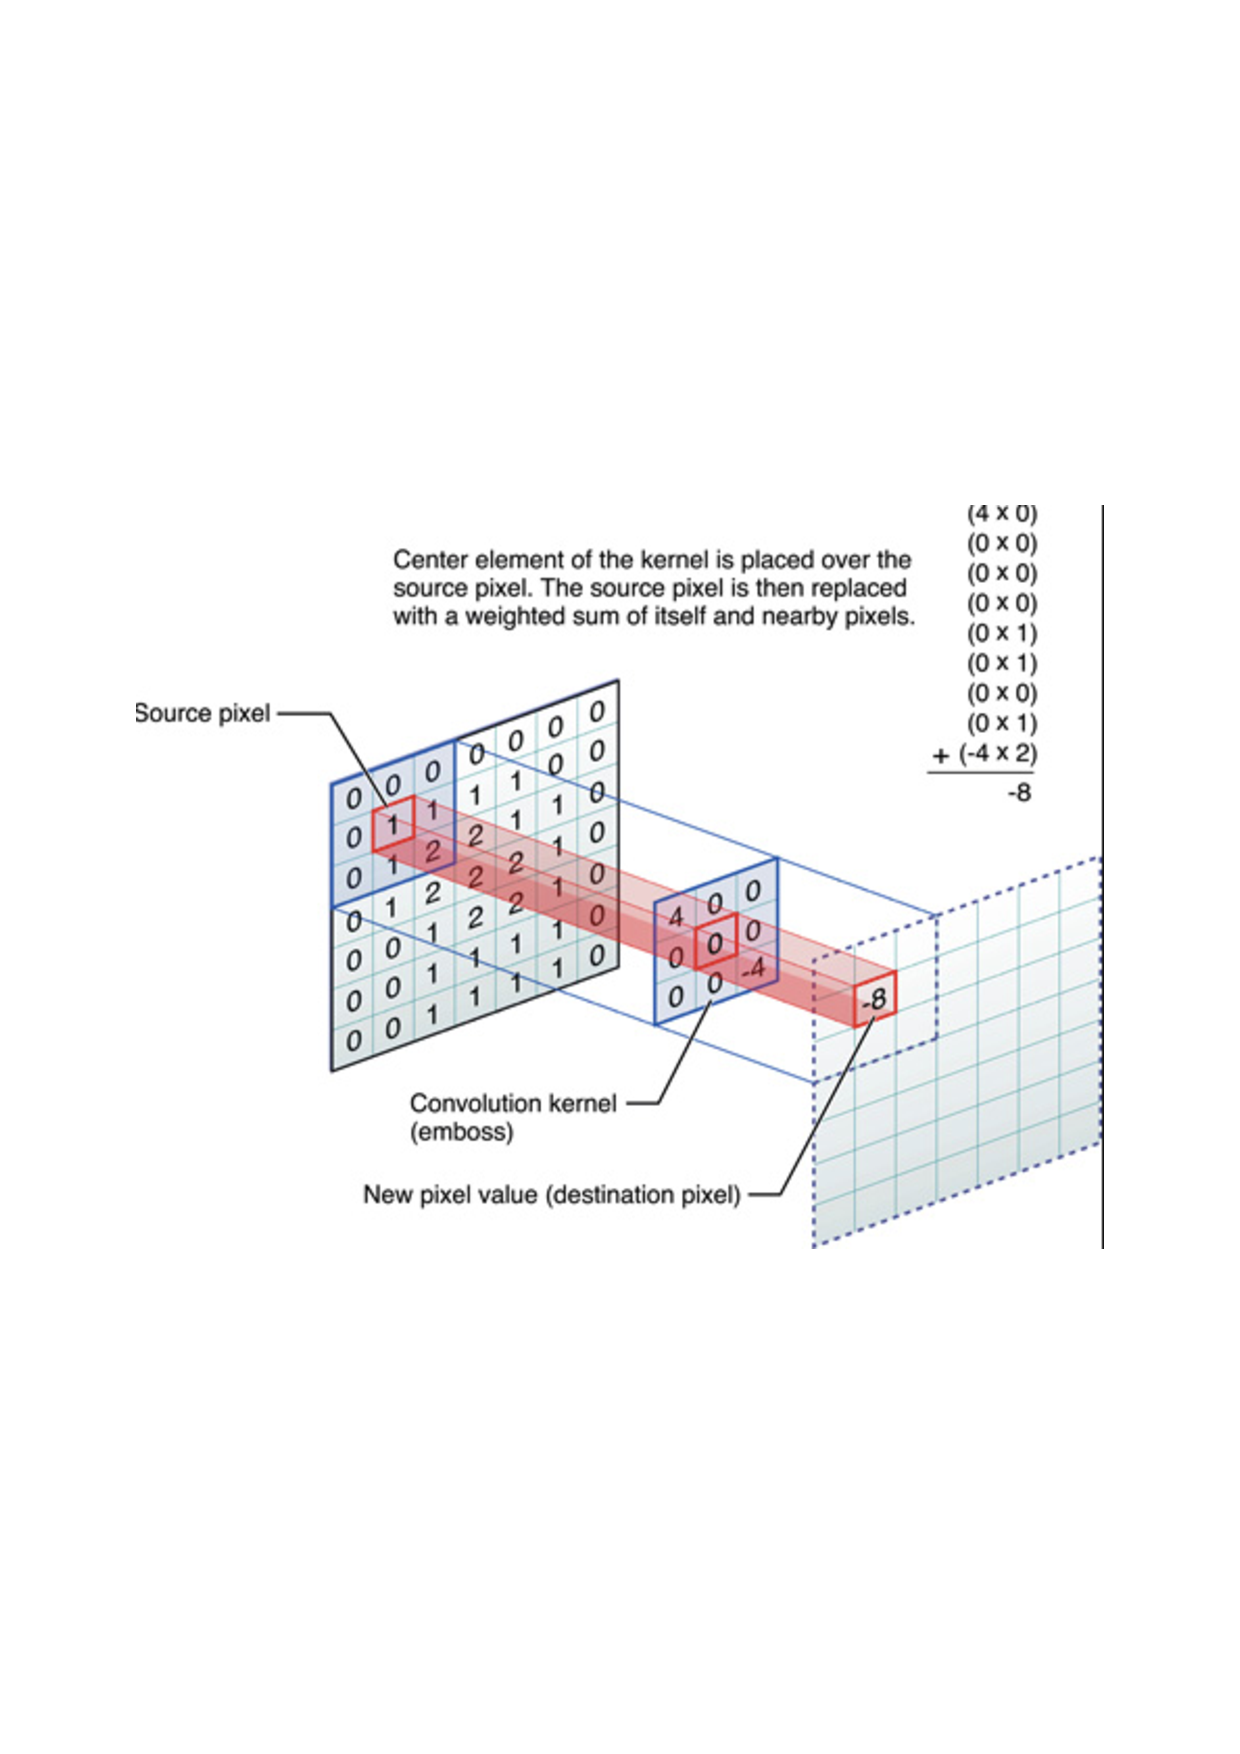
\includegraphics[trim=2cm 7cm 2cm 7cm, clip=true, height=80mm]{Chapter1/convolution.pdf}
\caption{The convolution layer. Illustration of the formation of a feature map.}
\end{figure}

The benefits of this approach are three folds :

\begin{itemize}
	\item sparse interaction: every output node is connected to a local subset of inputs instead of to all of of them.
	\item parameter sharing: the same kernel is used for every output node in a given feature map. 
	\item translational equivariance: shifting the input results in an equivalent shift in the output.
\end{itemize}

Every node in the feature map is then passed to an activation unit which non-linearly transforms the output from that node, thereby introducing some non-linearity into the system. These activation units usually consist of either a Tanh unit or a Rectified Linear Unit (ReLU) 

\subsection{Pooling Layer}

The pooling layer reduces the output with a local summary statistic such as the maximum or the average. This reduces the layer size and adds local translational invariance.

\begin{figure}
\centering
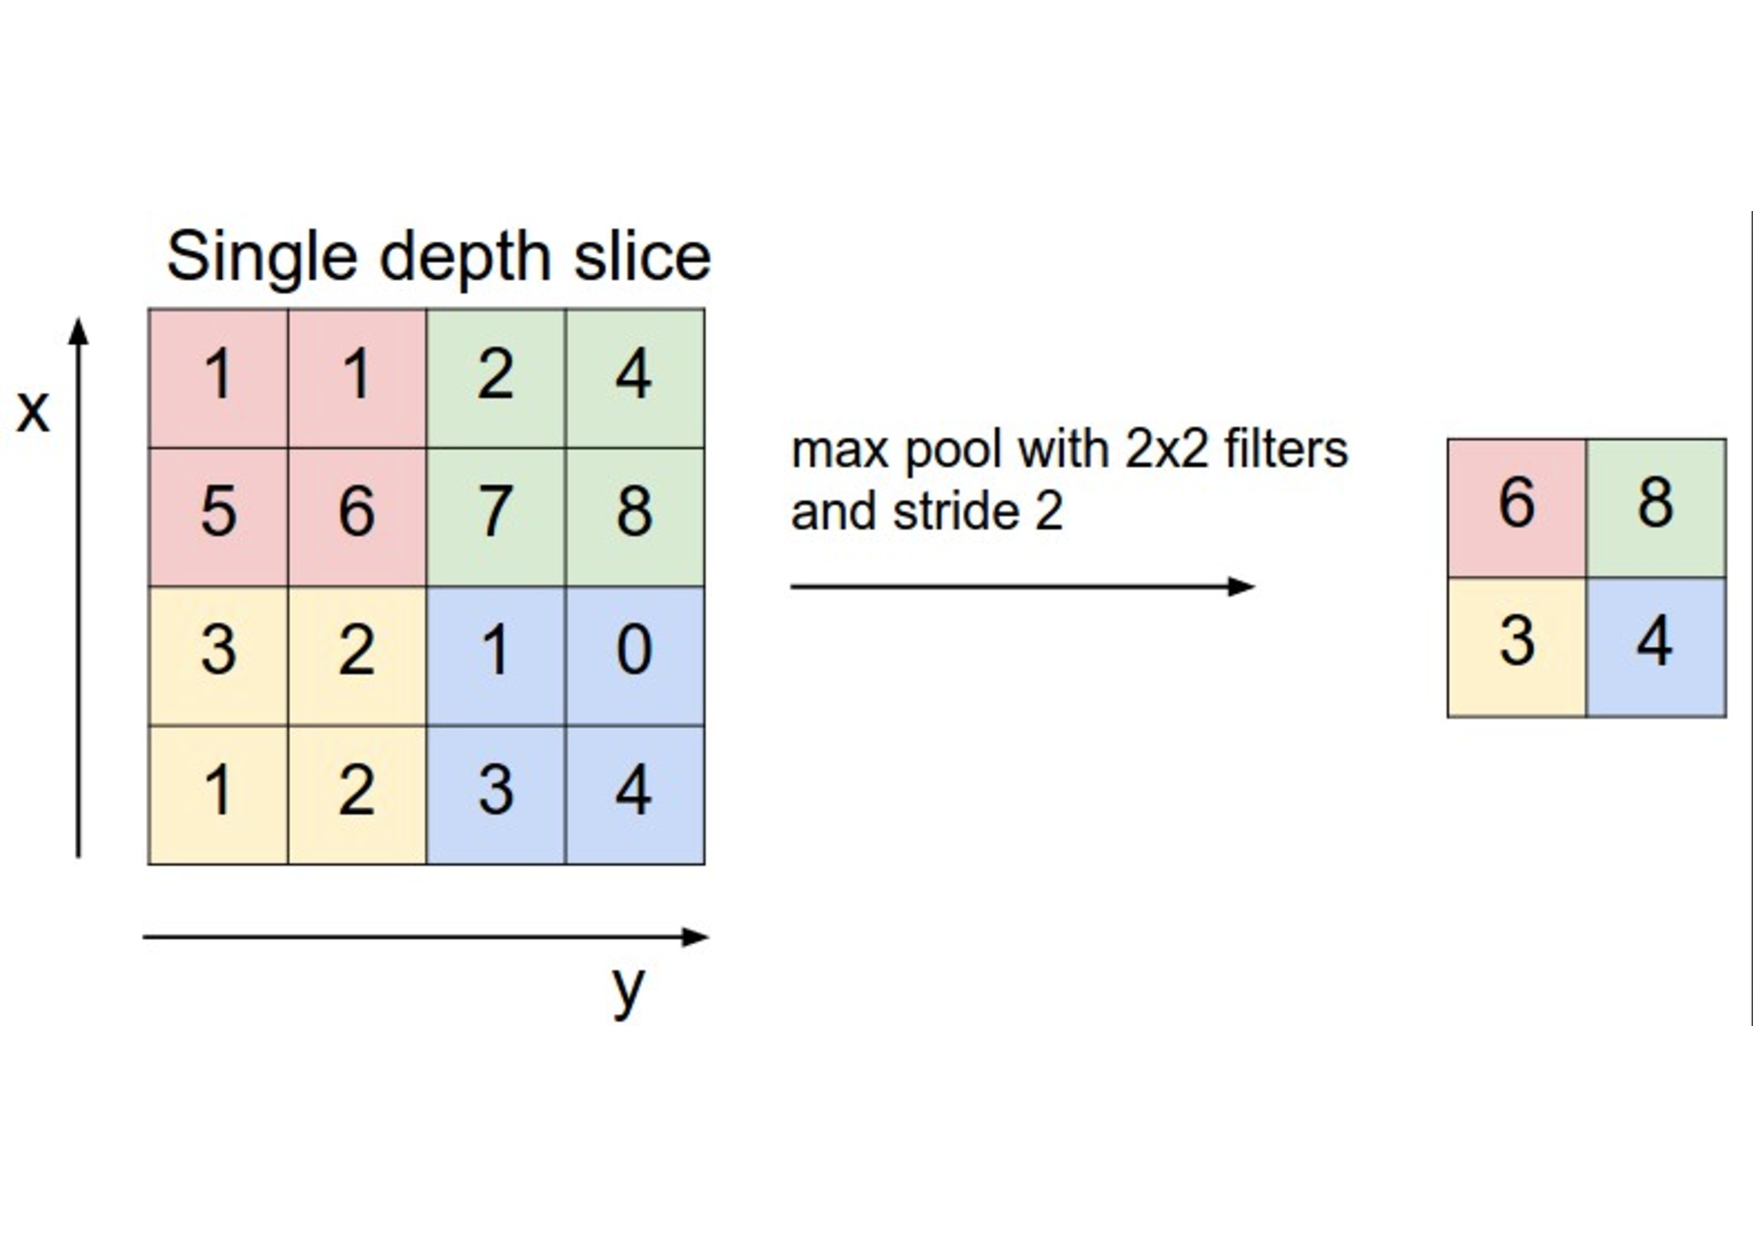
\includegraphics[trim=0cm 0cm 0cm 0cm, clip=true, height=60mm]{Chapter1/pooling.pdf}
\caption{The convolution layer. Illustration of the formation of a feature map.}
\end{figure}

\subsection{Typical Architecture}

A typical convolutional neural network architecture consists of an input layer, a number of convolutional layers, a number of fully connected layers, followed by an output layer. Each layer in turn are combinations of the nodes of the previous layer thus representing more abstract features the deeper its location in the architecture.



